\chapter{Boltzmann统计}

\section{理想气体}
\label{sec:ideal gas}

本节讨论满足非简并条件的理想气体，采用半经典Boltzmann分布。以单粒子基态为能量零点时，非简并要求$\e^\alpha \gg 1$。在计算分子气体的热容时，以下将质心平动(translation)、分子振动(vibration)和整体转动(rotation)近似为相互独立的运动。

\subsection{平动}
\label{ssec:translation}

由\exmref{exm:monatomic molecule}，单个粒子的平动能量和态密度为
\begin{subequations}
	\label{eq:sm-translational-state-density}
	\begin{align}
		\varepsilon_\transl &= \frac1{2m}(p_x^2 + p_y^2 + p_z^2),\\
		g(\varepsilon) &= \frac{2\pi V}{h^3}(2m)^{3/2}\sqrt\varepsilon.
	\end{align}
\end{subequations}
在能量准连续的条件下，配分函数
\begin{equation}
	Z_\transl = \intRplus g(\varepsilon)\e^{-\beta\varepsilon}\d\varepsilon = \frac{2\pi V}{h^3}(2m)^{3/2}\intRplus\sqrt\varepsilon\e^{-\beta\varepsilon}\d\varepsilon = V\biggp{\frac{2\pi m}{h^2\beta}}^{3/2}.
\end{equation}
考虑只有平动的情况，如单原子分子，
\footnote{统计力学部分，$n := N/V$表示粒子数密度，而不再表示摩尔数。}
\[
	\e^{\alpha} = \frac{Z_\transl}N = \frac1n\biggp{\frac{2\pi m\kB T}{h^2}}^{3/2},
\]
说明在稀薄、高温、大质量的情况下，$\e^\alpha \gg 1$，满足非简并条件。
另外，非简并条件也可以写成$\e^{-\alpha} = n\lambda_T^3 \ll 1$的形式，
其中$\lambda_T$是能量为$\pi\kB T$时的de Broglie波长
\begin{equation}
	\label{eqn:de Broglie wavelength}
	\lambda_T = \frac{h}{\sqrt{2\pi m\kB T}}.
\end{equation}
基于配分函数，可得平动所贡献的内能、比热、压强和熵：
	\footnote{全同气体粒子的配分函数含有置换因子$1/N!$，其对熵的贡献保证了下式的广延性。}
\begin{subequations}
	\begin{align}
		U_\transl &= -N\pv{\ln Z_\transl}\beta = \frac32N\kB T,\\
		C_{V,\transl} &= \pvat{U_\transl}{T}{V} = \frac32N\kB,\\
		p &= \frac N\beta\pv{\ln Z_\transl}V = \frac{N\kB T}V,\\
		S_\transl
		% &=N\kB\biggp{\ln Z_\transl-\beta\pv{\ln Z_\transl}\beta-\ln N+1}\\
		&= \frac52N\kB + N\kB\ln\biggb{\frac VN\biggp{\frac{2\pi m\kB T}{h^2}}^{3/2}}.
	\end{align}
\end{subequations}
将状态方程$pV = N\kB T$与实验得到的理想气体状态方程\eqref{eqn:pV=nRT}对比，可得理想气体常数$R = \kB\NA$。
由于国际单位制直接指定了$\kB$和$\NA$的值，因此$R$的数值也是精确的。

\begin{theorem}
	{Maxwell速度分布律}{Maxwell distribution of velocities}
	速率在$(v,v + \d v)$范围内的粒子数密度为
	\begin{equation}
		f(v)\d v = 4\pi n\biggp{\frac m{2\pi\kB T}}^{3/2}\e^{-mv^2/2\kB T}v^2\d v.
	\end{equation}
	\begin{notecaptionblock}
		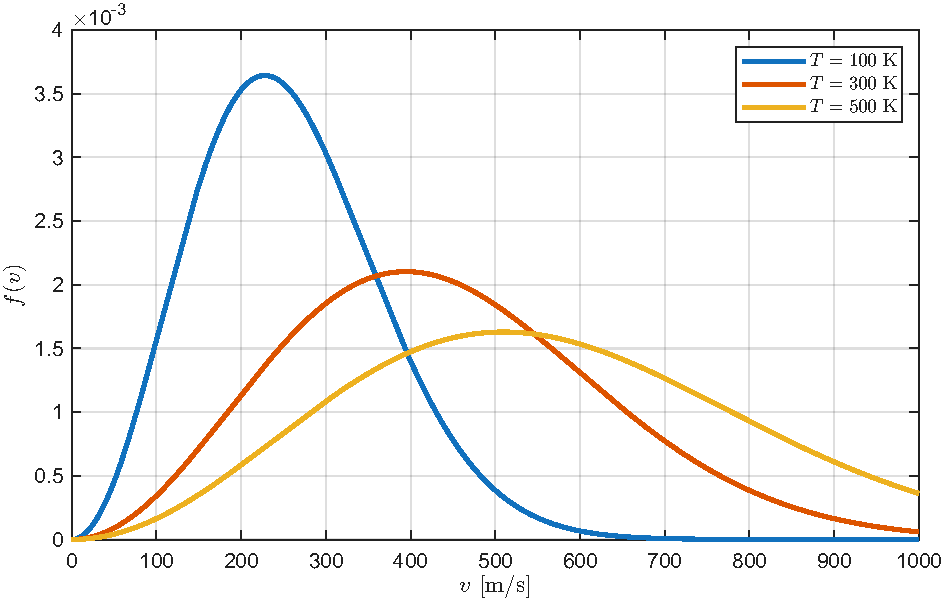
\includegraphics[width=0.8\linewidth]{figures/Maxwell_distribution.pdf}
		\captionof{figure}{氧气分子的 Maxwell 速率分布。纵轴为概率密度 $p(v) = f(v)/n$，其对速率的积分为 1。}
		\label{fig:Maxwell distribution}
	\end{notecaptionblock}
\end{theorem}

\begin{proof}
	动量在$\d p = \d p_x\nd p_y\nd p_z$范围内的粒子数密度为
	\[
		\e^{-\alpha-\beta\varepsilon}\frac{\d p}{h^3} = \frac n{(2\pi m\kB T)^{3/2}}\e^{-\beta(p_x^2+p_y^2+p_z^2)/2m}\d p_x\nd p_y\nd p_z,
	\]
	由$p_i = mv_i$，可得
	\begin{equation}
		f(v_x,v_y,v_z)\d v_x\nd v_y\nd v_z = n\biggp{\frac m{2\pi\kB T}}^{3/2}\e^{-m(v_x^2+v_y^2+v_z^2)/2\kB T}\d v_x\nd v_y\nd v_z.
	\end{equation}
	易证，$f(v_x,v_y,v_z)$是归一化的：
	\[
		\intR\intR\intR f(v_x,v_y,v_z)\d v_x\nd v_y\nd v_z = n.
	\]
	将坐标$(v_x,v_y,v_z)$换为球坐标$(v,\theta,\phi)$，并对$\theta,\phi$直接积分，便得到速率的分布。
\end{proof}

\begin{corollary}
	最概然速率$v_\mostprobable$、平均速率$\ave v$和方均根速率$v_\mathrm s$为
	\begin{subequations}
		\begin{align}
			v_\mostprobable &= \sqrt{\frac{2\kB T}m},\\
			\ave v &= \sqrt{\frac{8\kB T}{\pi m}},\\
			v_\mathrm s &= \sqrt{\frac{3\kB T}m}.
		\end{align}
	\end{subequations}
	取$x$轴正向指向器壁，单位时间碰撞单位面积器壁的粒子数为
	\begin{equation}
		\Gamma = \int_{v_x>0} v_x f(v_x,v_y,v_z)\,\d^3v = \frac14n\ave v.
	\end{equation}
\end{corollary}

\subsection{振动}
\label{ssec:vibration}

考虑一维振动，%取约化质量$\mu$，
有
\[
	\varepsilon_\vib = h\nu\biggp{n + \frac12},\quad\omega_\vib = 1.
\]
能量间距$\Delta\varepsilon_\vib = h\nu \sim \qty{0.1}{\electronvolt} > \qty{0.025}{\electronvolt}$常温，因此必须考虑能级的分立性。
定义振动的特征温度
\begin{equation}
	\label{eq:sm-vibrational-temperature}
	\theta_\vib := \frac{\Delta\varepsilon_\vib}\kB = \frac{h\nu}\kB \sim \qty{e3}{\kelvin}.
\end{equation}
则配分函数
\begin{equation}
	Z_\vib = \sum_n\omega_\vib\e^{-\beta\varepsilon_\vib} = \sum_{n=0}^\infty\e^{-(n+1/2)\beta h\nu} = \frac{\e^{-\beta h\nu/2}}{1 - \e^{-\beta h\nu}}.
\end{equation}
内能和比热
\begin{subequations}
	\begin{align}
		U_\vib &= -N\pv{\ln Z_\vib}\beta = Nh\nu\biggp{\frac12 + \frac1{\e^{\beta h\nu} - 1}},\\
		C_{V,\vib} &= \pvat{U_\vib}{T}{V} = N\kB\Einstein\biggp{\frac{\theta_\vib}T}.
	\end{align}
\end{subequations}
其中Einstein函数
\begin{equation}
	\label{eq:sm-einstein-function}
	\Einstein(x) := \frac{x^2\e^x}{(\e^x - 1)^2} =
	\begin{cases}
		1 - \frac{x^2}{12} + \bigo(x^4),&x \ll 1,\\
		x^2\e^{-x} + \bigo(x^2\e^{-2x}),&x \gg 1.
	\end{cases}
\end{equation}
分别对应高温和低温极限。高温极限下，能量准连续，$U_\vib = N\kB T$，比热$C_{V,\vib} = N\kB$；而在低温极限下，比热
\begin{equation}
	C_{V,\vib} \simeq N\kB\biggp{\frac{\theta_\vib}T}^2\e^{-\theta_\vib/T},\quad T \ll \theta_\vib.
\end{equation}

\begin{notecaptionblock}
	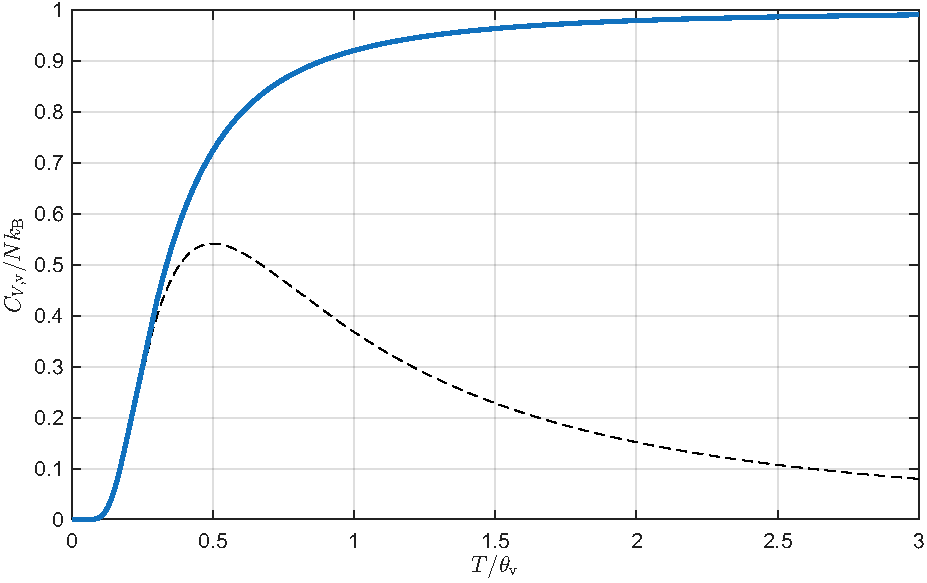
\includegraphics[width=0.8\linewidth]{figures/C_Vvib.pdf}
	\captionof{figure}{振动热容的 $C_{V,\vib}/(N\kB)\vs T/\theta_\vib$ 曲线}
	\label{fig:C_Vvib - T}
\end{notecaptionblock}

\begin{example}
	{Einstein固体热容模型}{Einstein solid heat capacity model}

	讨论固体晶格振动对$C_V$的贡献。
	晶格间强耦合，当$T$不太高时，振幅小，晶格振动可约化为$3N$个独立、可区别的简谐振动。
	Einstein假设振动频率$\nu_i = \nu$是一样的，
	\[
		\varepsilon_n = h\nu\biggp{n + \frac12},\quad n = 0,1,2,\ldots
	\]
	和前面理想气体的振动类似，可得热容
	\begin{equation}
		\label{eq:sm-einstein-heat-capacity}
		C_V = 3N\kB\Einstein\biggp{\frac{\theta_{\Einstein}}T},
	\end{equation}
	其中Einstein温度$\theta_{\Einstein} = h\nu/\kB \sim \qtyrange{100}{300}{\kelvin}$。
	在低温下$C_V \propto T^{-2}\e^{-\theta_{\Einstein}/T}$与实验定性相符，定量不符。
	因为有低频模式在低温时仍能被激发，从而对$C_V$有贡献。(见Debye模型)

\end{example}

平动动能含三个动量二次项。一维简谐振动有一个振动自由度，其能量含动能和势能两个二次项。这解释了经典极限下$U_\transl = 3N\kB T/2$、$U_\vib = N\kB T$。

\begin{theorem}{能量均分定理}{energy equipartition}
	在经典正则分布中，若广义坐标或动量$x$取遍实轴，且在Hamilton量中只以独立二次项$Ax^2$出现（$A > 0$），则该项的平均能量为$\kB T/2$。
\end{theorem}

\begin{proof}
	由正则权重分部积分，边界项$x\e^{-\beta Ax^2}$在两端均为零，因此
	\[
		\ave{Ax^2} = -\frac{1}{2\beta}
		\frac{\intR x\,\d(\e^{-\beta Ax^2})}{\intR\e^{-\beta Ax^2}\d x}
		= \frac1{2\beta} = \frac12\kB T.\qedhere
	\]
\end{proof}

\begin{remark}
	对具有分立能级的运动，$\kB T$远大于相关能级间距时才可用经典近似。通常的分子气体中，电子和原子核激发所需的能量远大于$\kB T$，因而这些激发对热容的贡献很小。
\end{remark}

\subsection{转动}
\label{ssec:rotation}

以异核双原子分子\footnote{同核分子还要满足核交换对称性。以电子基态的$\mathrm H_2$为例，正氢的两个质子组成总核自旋$I_{\rm nuc} = 1$的对称三重态，只允许奇数$\ell$。仲氢的总核自旋$I_{\rm nuc} = 0$，为反对称单态，只允许偶数$\ell$。}为例，
\begin{equation}
	\label{eq:sm-rotor-spectrum}
	\varepsilon_\rot = \frac{\hbar^2}{2I}\ell(\ell + 1),\quad\omega_\rot = 2\ell + 1.
\end{equation}
转动特征温度
\begin{equation}
	\label{eq:sm-rotational-temperature}
	\theta_\rot = \frac{\hbar^2}{2I\kB} \sim \qty{10}{\kelvin}.
\end{equation}
高温下，能量准连续，可得内能$U_\rot = N\kB T$，比热$C_{V,\rot} = N\kB$符合能量均分定理；
低温下，可按转动量子数依次写出配分函数的各项，
\begin{equation}
	\label{eq:sm-rotor-partition}
	Z_\rot = \sum_{\ell=0}^\infty(2\ell + 1)\e^{-\ell(\ell+1)\theta_\rot/T} = 1 + 3\e^{-2\theta_\rot/T} + 5\e^{-6\theta_\rot/T} + \bigo(\e^{-12\theta_\rot/T}).
\end{equation}
只考虑$\ell = 0,1$两项，可得
\begin{subequations}
	\begin{align}
		U_\rot &\simeq 6N\kB\theta_\rot\e^{-2\theta_\rot/T},\\
		C_{V,\rot} &\simeq 12N\kB\biggp{\frac{\theta_\rot}T}^2\e^{-2\theta_\rot/T}.
	\end{align}
\end{subequations}
在任意正温下，按单分子转动配分函数取平均，有$C_{V,\rot}/(N\kB) = \beta^2(\ave{\varepsilon_\rot^2} - \ave{\varepsilon_\rot}^2)$。\figref{fig:C_Vrot - T}中的热容在$T \simeq 0.807\theta_\rot$处达到$1.098N\kB$，随后从上方趋于经典值$N\kB$。

\begin{notecaptionblock}
	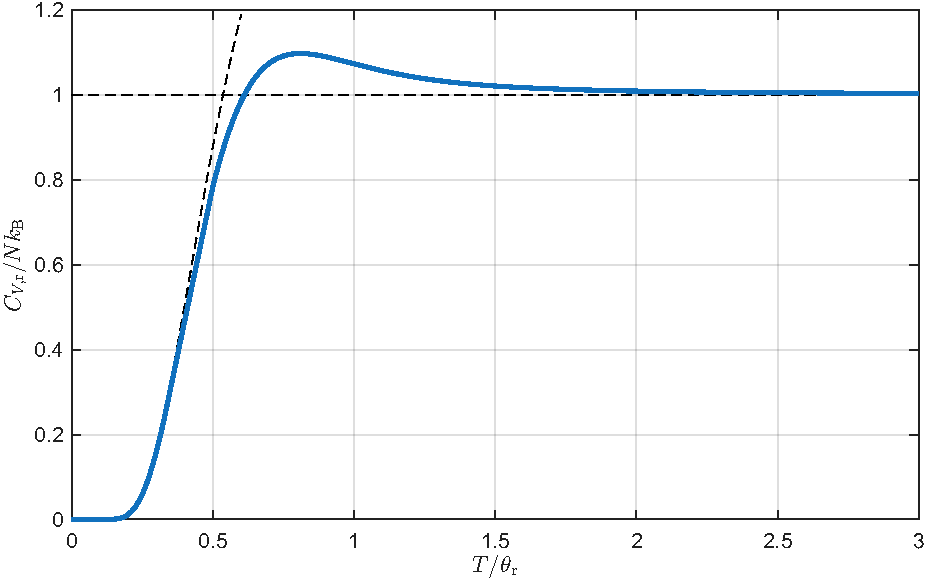
\includegraphics[width=0.8\linewidth]{figures/C_Vrot.pdf}
	\captionof{figure}{转动热容的 $C_{V,\rot}/(N\kB)\vs T/\theta_\rot$ 曲线}
	\label{fig:C_Vrot - T}
\end{notecaptionblock}

总的内能和热容就是三种独立运动的和：
\[
	C_V = C_{V,\transl} + C_{V,\rot} + C_{V,\vib}.
\]
在上述双原子分子模型中，取与氧气相近的特征温度$\theta_\rot = \qty{2.40}{K}$、$\theta_\vib = \qty{2230}{K}$，并对所有非负整数$\ell$求和。随着转动、振动相继被激发，\figref{fig:C_V - T} 中的热容依次接近$3N\kB/2$、$5N\kB/2$和$7N\kB/2$。实际的$^{16}\mathrm{O}_2$在电子基态只允许奇数转动量子数，计算其低温热容需使用相应的分子能级。

\begin{notecaptionblock}
	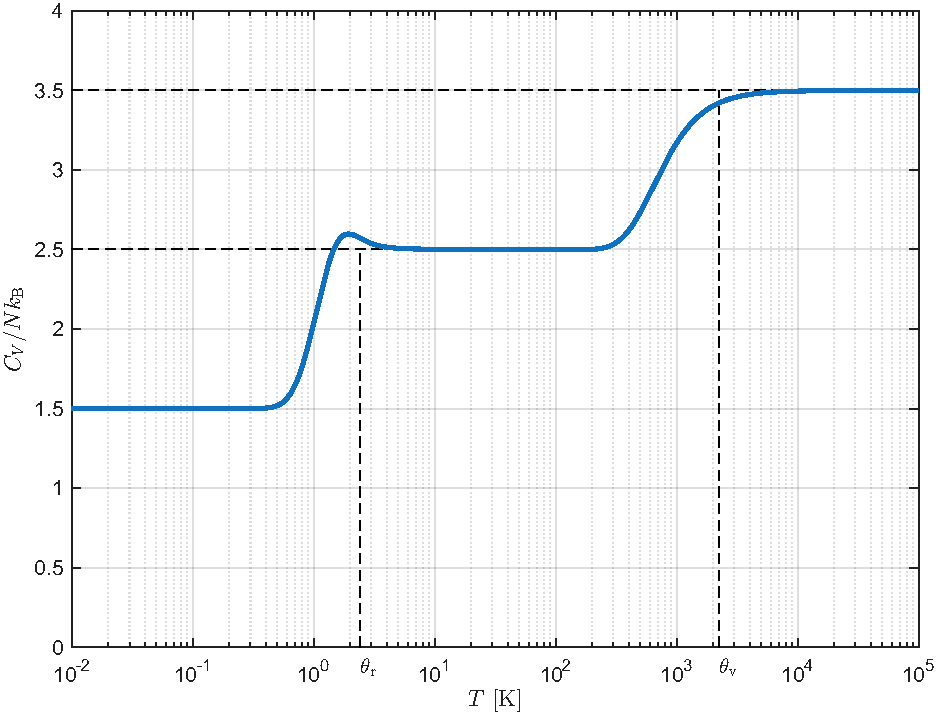
\includegraphics[width=0.8\linewidth]{figures/C_Vtot.pdf}
	\captionof{figure}{双原子分子模型的总热容随温度的变化}
	\label{fig:C_V - T}
\end{notecaptionblock}

\section{顺磁性物质}

考虑由相互作用可忽略的原子磁矩组成的顺磁体。在给定的总角动量多重态内，电子的有效磁矩与总角动量$\bm J = \bm L + \bm S$之间满足
\[
	\bm\mu = -g\muB\frac{\bm J}{\hbar},
\]
其中$\muB := e\hbar/(2m_\electron)$为Bohr磁子。对满足$LS$耦合、$j > 0$的多重态，取电子自旋$g$因子为2，Landé因子为
\begin{equation}
	\label{eq:sm-lande-factor}
	g = 1 + \frac{j(j + 1) + s(s + 1) - \ell(\ell + 1)}{2j(j + 1)}.
\end{equation}
取外加磁场$B = \mu_0 H$沿$z$方向，以$m = \mu_z/(g\muB)$标记磁矩的取向。忽略局域场修正，单个粒子的能量为
\begin{equation}
	\label{eq:sm-zeeman-levels}
	\varepsilon_m = -\mu_z B = -g\muB Bm,\qquad m = -j,-j + 1,\ldots,j.
\end{equation}
单粒子配分函数为
\begin{equation}
	Z = \sum_{m=-j}^j\e^{-\beta\varepsilon_m} = \frac{\e^{aj} - \e^{-a(j+1)}}{1 - \e^{-a}} = \Biggdivision{\sinh\biggb{\biggp{j + \frac12}a}}{\sinh\frac a2}.
\end{equation}
其中$a := \beta\mu_0\muB gH$。
用$n = N/V$表示磁矩的数密度。沿外场方向的磁化强度$M$为单位体积的平均磁矩，系统的总磁矩为$VM$。由单粒子配分函数得到
\begin{subequations}
	\begin{align}
		M &= \frac n\beta\pvat{\ln Z}{B}{T} = n\muB gj\Brillouin_j(a),\\
		U &= -N\pvat{\ln Z}{\beta}{B} = -BVM.
	\end{align}
\end{subequations}
此处$U$是包含Zeeman能的自旋Hamilton量的平均值，其磁功项为$-VM\,\d B$。\chapref{chap:simple system}采用磁功$B\,\d m$，其中$m = VM$；将该章的内能作变换$U \mapsto U - Bm$即得这里的能量约定。
式中的Brillouin函数为
\begin{equation}
	\label{eq:sm-brillouin-function}
	\Brillouin_j(a) := \frac1j\biggB{\biggp{j + \frac12}\coth\biggb{\biggp{j + \frac12}a} - \frac12\coth\frac a2}.
\end{equation}
\begin{notecaptionblock}
	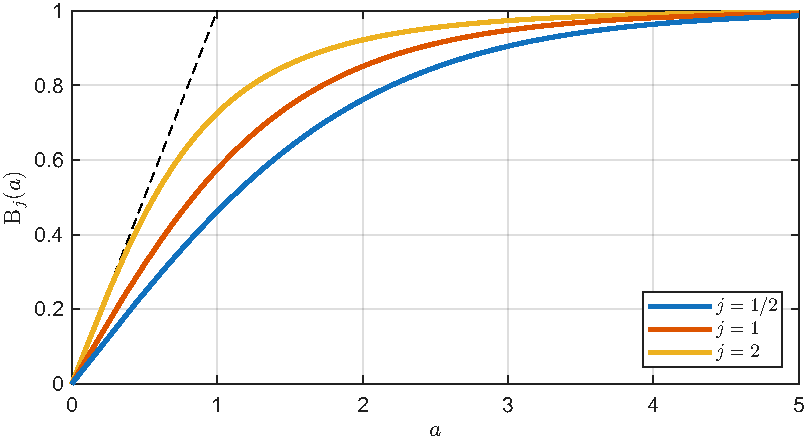
\includegraphics[width=0.8\linewidth]{figures/Brillouin.pdf}
	\captionof{figure}{Brillouin函数$\Brillouin_j(a)$}
	\label{fig:Brillouin function}
\end{notecaptionblock}

高温弱场极限下，$(j + 1/2)\abs a \ll 1$，由$\coth$展开式可得
\[
	\Brillouin_j(a) = \frac{j + 1}3a - \frac{(j + 1)(2j^2 + 2j + 1)}{90}a^3 + \bigo(a^5).
	% \Brillouin_j(a)=\frac{j+1}3a-\frac{(j+1)[j^2+(j+1)^2]}{90}a^3+\frac{(j+1)[3j^2+(j+1)^2][j^2+3(j+1)^2]}{7560}a^5+\bigo(a^5).
\]
仅保留一阶项，
可得
\[
	M \simeq \frac{n\mu_0\muB^2g^2j(j + 1)}{3\kB T}H.
\]
\begin{theorem}
	{Curie定律}{Curie's Law}
	在弱场极限下，磁化强度$M = \chi H$与外场强度$H$成正比，体磁化率$\chi$与绝对温度成反比：
	\begin{equation}
		\chi = \frac{n\mu_0\muB^2g^2j(j + 1)}{3\kB T} \propto \frac1T.
	\end{equation}
\end{theorem}
低温强场极限下，$a \gg 1$，$\Brillouin_j(a) \simeq 1$
\[
	M \simeq n\muB gj.
\]
代表所有磁矩都与外场平行，达到饱和。

\paragraph{绝热退磁}

考虑Helmholtz自由能和熵
\begin{align*}
	F &= -\frac N\beta\ln Z =: \frac1\beta\phi(\beta H),\\
	S &= -\pv FT = \kB[-\phi(\beta H) + \beta H\phi'(\beta H)].
\end{align*}
在磁矩间相互作用和晶格热容均可忽略的温区，可逆绝热过程保持自旋熵不变，因此$\beta H = \const$。
即当外场$H$下降时，温度$T$也会下降，并且满足
\begin{equation}
	\label{eq:sm-adiabatic-demagnetization}
	T_\final = T_\initial\frac{H_\final}{H_\initial}.
\end{equation}
为实现这一效果，可选取$S(H = 0)$随温度变化小的物质，比如$\mathrm{Ce_2Mg_3(NO_3)_{12}\cdot(H_2O)_{24}}$。

\section{负绝对温度}

1956年，Ramsey提出了有关负绝对温度的热力学与统计理论。根据
\[
	\frac1T = \pvat{S}{U}{V,N},
\]
一般情况下，内能越高，可能的微观状态数越多，熵越大，温度为正。但也有例外，这使负绝对温度的实现成为可能。

\paragraph{核自旋系统}

在固定外磁场$B$下，考虑自旋量子数为$1/2$的核，其磁矩的两个投影对应能量$\pm\varepsilon$。取$\varepsilon > 0$，
记两种取向的核磁矩数为$N_\pm$，
由系统的粒子数和能量关系：
\[
	\begin{cases}
		N = N_+ + N_- \\
		U = (N_+ - N_-)\varepsilon
	\end{cases}
	\implies
	N_\pm = \frac N2\biggp{1 \pm \frac U{N\varepsilon}}.
\]
微观状态数$\Omega = N!/(N_+!N_-!)$，
熵
\begin{align*}
	S & = \kB\ln\biggp{\frac{N!}{N_+!N_-!}} \simeq \kB(N\ln N - N_+\ln N_+ - N_-\ln N_-).
	  \\ & = N\kB\biggb{\ln 2 - \frac12\biggp{1 + \frac U{N\varepsilon}}\ln\biggp{1 + \frac U{N\varepsilon}} - \frac12\biggp{1 - \frac U{N\varepsilon}}\ln\biggp{1 - \frac U{N\varepsilon}}}
\end{align*}
故温度的倒数
\begin{equation}
	\frac1T = \pvat{S}{U}{B,V,N} \simeq \frac\kB{2\varepsilon}\ln\biggp{\frac{N_-}{N_+}}
	\begin{cases}
		> 0,&N_- > N_+\\
		< 0,&N_- < N_+
	\end{cases}
\end{equation}
当能量$U$从负转正的过程中，绝对温度的变化为
\[
	+T_0\enspace \longrightarrow \enspace +\infty\enspace \to \enspace -\infty\enspace \longrightarrow \enspace -T_0
\]
\begin{notecaptionblock}
	\tikzfigure{spin-temperature}
	\captionof{figure}{$T\vs N_+$图像}
\end{notecaptionblock}

\begin{remark}
	实现负绝对温度的条件相当苛刻：
	\begin{compactenum}
		\item 系统的能量$U$有上界；
		\item 系统内部实现平衡（系统能与环境隔绝一段时间）。即
		\begin{center}
			系统内部弛豫时间$\ll$系统与环境之间的弛豫时间
		\end{center}
		对于LiF晶体，前者为$\qty{e-5}{\second}$，后者为$\qty{5}{\minute}$。
		1951年，Purcell和Pound在很纯的LiF晶体的核自旋系统中实现了负绝对温度的状态。
	\end{compactenum}
	只有满足以上条件，划分才有意义。
\end{remark}

